\documentclass[a4paper,12pt]{report}
\usepackage[utf8]{inputenc}
\usepackage[T1]{fontenc}
\usepackage[english]{babel}
\usepackage{lmodern}
\usepackage{microtype}
\usepackage{amsmath,amsthm}
\usepackage{amsfonts}
\usepackage{amssymb}
\usepackage{graphicx}
\usepackage{hyperref}
\usepackage{textpos}
\usepackage{dirtytalk}
\usepackage{fancyhdr}
\usepackage[nottoc]{tocbibind}
\usepackage{float}
\usepackage{enumitem}
\usepackage{tikz}
\usepackage{geometry}
\usepackage{array}
\usepackage[pages=some]{background}
\usepackage{mathrsfs}
\usepackage{algorithm}
\usepackage{algorithmic}
\usepackage{longtable}
\usepackage{tikz}
\usetikzlibrary{calc}
\usepackage{multirow}
\usepackage{makecell}
\usepackage{amsmath}
\usepackage{indentfirst}
\usepackage{caption}
%\captionsetup[table]{position=bottom}
\usepackage{siunitx}
\usepackage{titlesec}
\setcounter{secnumdepth}{4}   
  
 



% For dummy lipsum text
\usepackage{lipsum}

\usepackage{hyperref}
\hypersetup{ colorlinks,citecolor=blue,filecolor=blue,linkcolor=blue, urlcolor=blue}
\numberwithin{equation}{section}


\begin{document}
\title{Streamlined Hotel Room Reservation Web App }
\author{Abidi Ranim}
\date{Academic year 2021-2022}

%régler l'espacement entre les lignes
\newcommand{\HRule}{\rule{\linewidth}{0.6mm}}

%page de garde
\backgroundsetup{
scale=1,
color=black,
opacity=1,
angle=0,
contents={%
  
\includegraphics[width=19cm,height=28cm]{images/background.png}
  }%
}

\begin{titlepage}
\BgThispage
\begin{textblock}{4}[0.55,0.5](1,0.15)
	
\includegraphics[width=\linewidth]{images/isik.png}\\[2cm]
  \end{textblock}
  
\begin{textblock}{2.0}[0.25,0.5](10,0.5)
	
\includegraphics[width=\linewidth]{images/uj.png}\\[3.5cm]
  \end{textblock}
  
  
%\newline
\bigskip
\bigskip
\begin{center}
{ \large{HIGHER INSTITUTE OF COMPUTER SCIENCE OF KEF }}\\[0.5cm]
{ \large{University of Jendouba, Tunisia}}\\[0.8cm]
{\large{Computer Science Department}}\\[0.5cm]
{\large \textbf{Year-end project}}\\[0.3cm]

% Title
\rule{\linewidth}{0.5mm} \\[0.5cm]
{ \huge \bfseries 
Transfer Management System 
}
\rule{\linewidth}{0.5mm} \\[0.5cm]

% Author and supervisor
\noindent
\begin{center}\large
    \emph{ Prepared by :}\\[0.5cm]
  \textbf{Mohamed Aziz Jbeli}  \\[0.5cm]      {\large 2nd~year Software Engineering }\\[0.5cm] 
 \bigskip 
  \emph{Supervised by : }\\[0.5cm]
  \textbf{Mr. }
\bigskip    
\bigskip
\bigskip

  \emph{Organization:}\\[0.5cm]
  \begin{figure}[H]
   \centering
    %\includegraphics[scale=0.5]{images/trasfvs.jpg}
    
\includegraphics[width=4.0cm,height=3.0cm]{images/hotel.png}
\end{figure}

\vfill {\small Academic year: 2023/2024}\\
\end{center}


% Bottom of the page

\end{center}

\end{titlepage}



%page blanche
%ne pas numéroter cette page
\pagenumbering{Roman}
\chapter*{Acknowledgements}
\addcontentsline{toc}{chapter}{Acknowledgements}
With these few words, I would like to pay tribute to all the people who have contributed to the good progress of this project and its accomplishment in the best conditions.\\

This work would not have been possible without the presence of my family mom, dad and my little brother, also, my supervisor Mr. Arbi Menzli and my professors at ISI KEF who were always motivating, helpful and responsive. Their valuable advice had spared no effort to transmit to me information and put me on the right track.\\

I would also like to thank the jury for having devoted their precious time to judge this work.


\begin{thankingpage}
\BgThispage
\begin{textblock}{8}[0.01,0.5](2.5,5)
	
\includegraphics[width=\linewidth]{images/sign.png}\\[2cm]
  \end{textblock}


\newpage

\begin{abstract}  

%\addcontentsline{toc}{section}{\numberline{}Abstract} 
%\addcontentsline{toc}{chapter}{Abstract}
In my work we started with a research about the  types of hotels websites , and then we started exploring the types of informations needed by the hotel. Afterwards, we went to the development part, where we prepared the programming language and the framework and then started the web development. \\



\end{abstract}

\newpage

\include{abstract1}               
\addcontentsline{toc}{chapter}{ Abstract}
\tableofcontents
\listoffigures


\newcommand{\RNum}[1]{\uppercase\expandafter{\romannumeral #1\relax}}





%ne pas numéroter le sommaire

%espacement entre les lignes d'un tableau
\renewcommand{\arraystretch}{1.5}

%====================== INCLUSION DES PARTIES ======================

%recommencer la numérotation des pages à "1"
%\addtocontents{toc}{\protect\enlargethispage{\baselineskip}}
%\onehalfspacing


\chapter*{List of Tables}
\addcontentsline{toc}{chapter}{List of Tables}
\color{Blue!} 

2.1 Textual description for the use case 'authenticate' . . .  . . . . . . . .  .. 10\\
2.2 Textual description for the use case 'process reservation' . . .. . . . . . . .. 10\\
2.3 Textual description for the use case 'add reservation'. . . . . . .  . . . ... . .. 11\\
2.4 Textual description for the use case 'Register'. . . . . . . . . . .. . . . . .  .. .  12\\
2.5 Textual description for the use case 'Consult reservation'. . . .  . . . . . .  . 12\\ 

 
\newpage
\color{Black!} 

\chapter*{General Introduction}
\addcontentsline{toc}{chapter}{General Introduction}
This internship has provided a very enriching path with information and experiences for the student to employ their skills in a professional and well-supported environment. Over the course of four weeks, we have managed to achieve our goals of gathering as much information as possible and using it appropriately in the creation of our web application.

The purpose of this report is not only to provide a comprehensive presentation of all the technical aspects that we have learned or deepened, but also, in a concise and clear manner, to give an overview of the technical and human aspects that we have encountered.

In this report, we first presented an overview of the project framework, then we presented the analysis and specification of requirements, followed by the design phase, and finally, the implementation phase.

 
\newpage


\pagenumbering{arabic}

\chapter{Project presentation}

\section{Introduction}
This current chapter is dedicated to giving a global overview of the project.  \\
This part presents the organization, including its problems , its difficulties , and the solution implemented .

\section{Presentation of the host organization  }

\subsection{The host organization introduction }
\begin{figure}[H]
   \centering
    %\includegraphics[scale=0.5]{images/trasfvs.jpg}
    
\includegraphics[width=6cm,height=6cm]{images/hotel.png}
    \caption{logo}
    \label{Samarons hotels logo}
\end{figure}
Exuding an aura of refined elegance and unsurpassed luxury, Samarons hotel epitomizes the pinnacle of opulent hospitality. With an unwavering commitment to impeccable service and an array of exclusive amenities, our distinguished establishment stands as a beacon of sophistication and comfort.  

\subsection{Organizational chart}

This is the structure of Samarons hotels :

\begin{enumerate}
\textbf{    \item General Manager:}
Overseeing the entire hotel operations, including the Computer Science department.

\textbf{    \item Computer Science Department:}

\begin{itemize}
\textbf{        \item Chief Technology Officer (CTO):}
Responsible for the overall technology strategy and implementation within the hotel.

        \item \textbf{IT Manager:}
Manages the hotel's IT infrastructure and oversees the Computer Science department's operations.

\textbf{        \item Software Development Team:}

    \begin{itemize}
            \item Development Manager
            \item Software Engineers/Developers
    \end{itemize}

\textbf{        \item Network and Systems Team:}

    \begin{itemize}
            \item Network Manager
            \item System Administrators
    \end{itemize}

\textbf{        \item Database Management Team:}

    \begin{itemize}
            \item Database Manager
            \item Database Administrators
    \end{itemize}

\textbf{        \item IT Support and Help Desk:}

    \begin{itemize}
            \item IT Support Manager
            \item IT Support Specialists
    \end{itemize}

\textbf{        \item Cybersecurity Team:}

    \begin{itemize}
            \item Cybersecurity Manager
            \item Cybersecurity Analysts
    \end{itemize}

\textbf{        \item Digital Marketing and E-Commerce Team:}

    \begin{itemize}
            \item Digital Marketing Manager
            \item E-Commerce Manager
    \end{itemize}

\textbf{        \item Technology Procurement and Vendor Management:}

    \begin{itemize}
            \item Procurement Manager
            \item Vendor Relationship Manager
    \end{itemize}

\end{itemize}

\textbf{    \item Rooms Division:}
Including roles such as Director of Rooms, Front Office Manager, and Housekeeping Manager.

\textbf{    \item Food and Beverage Division:}
Including roles such as Director of Food and Beverage, Executive Chef, Restaurant Manager, and Bar Manager.

\textbf{    \item Sales and Marketing:}
Including roles such as Director of Sales and Marketing, Sales Manager, and Marketing Manager.

\textbf{    \item Finance and Accounting:}
Including roles such as Director of Finance and Accounting Manager.

\textbf{    \item Human Resources:}
Including roles such as Director of Human Resources and Human Resources Manager.

\textbf{    \item Engineering and Maintenance:}
Including roles such as Director of Engineering and Maintenance Manager.

\textbf{    \item Security:}
Including roles such as Director of Security.

\end{enumerate}
 

\section{Existing analysis }

\textbf{1. Online Presence Analysis:}

The current analysis reveals that the hotel in question lacks any online presence, which severely limits its visibility within the competitive hospitality industry. This absence of a website hinders the hotel's ability to promote its services, showcase its amenities, and attract potential guests. Without an online platform, it is challenging for prospective clients to access crucial information such as room rates, available services, and the hotel's location.

\textbf{2. Competitor Analysis:}

A comprehensive study of the competitors in the same category or similar categories highlights that most hotels have well-designed and user-friendly websites. These websites provide features such as online booking, appealing photo galleries, detailed information about rooms and services, and customer testimonials. The online presence of competitors significantly contributes to their brand recognition, reputation, and customer acquisition.

\textbf{3. Reservation Channel Analysis:}

The hotel heavily relies on third-party reservation channels, such as online booking platforms (e.g., Booking.com, Expedia, etc.), due to the lack of its own website. This dependency can lead to high commissions and a loss of control over pricing policies and customer relationships. The absence of a direct reservation channel also limits the hotel's ability to establish a direct connection with its customers, making it challenging to personalize the guest experience and foster customer loyalty.

\textbf{4. Customer Feedback Analysis:}

Customer feedback analysis indicates that many clients face difficulties in obtaining accurate information about the hotel, including pricing, services offered, and room availability. Some guests express a preference for making direct reservations with the hotel instead of using intermediaries.

\textbf{5. Analysis of Potential Benefits:}

Implementing a website for the hotel offers numerous potential benefits, including increased visibility, improved control over pricing and room availability, enhanced guest experience, and the opportunity to establish direct relationships with customers. A well-designed website can also bolster the hotel's credibility and foster trust among potential clients.

 
\subsection{Description of the current situation }

The hotel suffers from a lack of visibility, a loss of control over reservations, and difficulties in establishing a direct relationship with its clientele due to the absence of a structured and effective online presence. The implementation of an optimized website thus represents a key opportunity to improve its competitive position and strengthen its relationship with customers.
\end{itemsize}

\subsection{Critique of the existing situation  }

The lack of an online presence for the hotel poses several significant challenges and drawbacks that hinder its competitiveness and customer reach in the modern digital landscape. Some critical points of critique include:

\begin{enumerate}
{        \item \textbf{Missed Marketing Opportunities:}}
The absence of a dedicated website deprives the hotel of crucial marketing opportunities to showcase its unique offerings, amenities, and services. This lack of visibility limits its ability to reach potential customers who primarily rely on online sources for hotel information and bookings.

\textbf{    \item Limited Customer Engagement:} 
Without a digital platform, the hotel struggles to engage with customers directly and provide personalized services. The inability to establish direct communication channels may lead to missed opportunities for tailored offerings, special promotions, and personalized customer experiences.

\textbf{    \item Dependence on Third-Party Channels:}
Relying solely on third-party booking channels often results in higher commission fees and reduced control over pricing strategies and customer data. This dependency can impact the hotel's revenue and profitability, limiting its ability to implement competitive pricing and tailored promotional campaigns.

\textbf{    \item Competitive Disadvantage:} 
In an industry where online presence is crucial, the hotel's lack of a website places it at a significant competitive disadvantage compared to other hotels that have well-established online platforms. Potential customers may overlook the hotel in favor of competitors with more accessible information and user-friendly booking processes.

\textbf{    \item Diminished Brand Image:}
The absence of a professional website can undermine the hotel's brand image and credibility in the eyes of potential customers. In the absence of an online platform, the hotel may struggle to establish a strong brand identity and may appear outdated or less reputable compared to competitors with robust online presences.

\textbf{    \item Inadequate Information Access:} 
Prospective guests may face challenges in obtaining comprehensive and accurate information about the hotel's amenities, room availability, and pricing. This lack of transparency and accessibility can deter potential customers and lead to missed business opportunities.

\end{enumerate}

\subsection{Proposed solution  }

To address the existing challenges and improve the hotel's competitiveness, the following solutions are proposed:

\begin{enumerate}
{        \item \textbf{Website Development:}}
Develop a user-friendly, visually appealing, and informative website that showcases the hotel's unique offerings, amenities, and services. Implement an intuitive user interface and ensure seamless navigation for an enhanced user experience.

\textbf{    \item Online Reservation System:}
Integrate a secure and efficient online reservation system directly on the hotel's website. This system should enable guests to check room availability, view pricing, and make direct bookings without the need for third-party booking platforms, thus reducing commission fees and improving the hotel's revenue stream.
\end{enumerate}
 
\section{Conclusion}
In this study,  the lack of an online presence for the hotel has significantly constrained its ability to compete effectively in the digital era of the hospitality industry. This absence has resulted in missed marketing opportunities, limited customer engagement, and a competitive disadvantage compared to other hotels with robust online platforms. Relying solely on third-party booking channels has also led to higher commission fees and reduced control over pricing strategies.
That's why we proposed the solution of a reservation and description website.
\chapter{Analysis and specification of needs }

\section{Introduction}

The success of any project depends on the quality of its outset. Therefore, the step of specifying the needs constitutes the starting base of our work; it must unequivocally describe the application to be developed. To ensure the expected objectives, it is essential that we achieve a clear view of the various anticipated needs of our project. In this chapter, we will identify the expected functionalities of the module by defining the various use cases. 

\section{Identification of stakeholders}

We start by identifying the actors involved in our solution. An actor is a person or component that interacts with the system. In our case, we have two actors:

\begin{itemize}
    \item The client: any individual
    \item The administrator: person responsible for the maintenance and 
        monitoring of a website or server on the Internet."
\end{itemize}
 \\
 
\section{Needs analysis }

\subsection{Functional needs analysis }

The analysis of functional needs translates the desired requirement by the client into functionalities achievable by our application.

The client can:

\begin{itemize}
    \item Register in the application
    \item Log into the application
    \item View reservation history
    \item Add a reservation
    \item Track the progress of reservation statuses
\end{itemize}
        The administrator can:

\begin{itemize}
    \item Log into the application
    \item Process reservations
    \item View reservations.

\end{itemize}

\subsection{The non-functional requirements }

Non-functional requirements represent the implicit requirements that the system must meet. For the proper functioning of our project, we have identified the following non-functional requirements:

\begin{itemize}
    \item \textbf{Usability:} ease of learning and use.
    \item \textbf{Efficiency:} it is imperative to minimize the processing time.
    \item \textbf{Utility:} the site must be efficient through its functionalities, and it 
        must meet all user requirements optimally. 
        \item \textbf{Extensibility:} the ease with which new functionalities can be added. 
\end{itemize}
 
\section{Modeling of requirements }

We have opted for the object-oriented method to specify our client's requirements. In this section, we present the use case diagrams.

\subsection{General use case diagram }

 The use case diagram highlights the interaction between the system and the various actors. Each use case designates a functionality of the system. 
\begin{figure}[H]
   \centering
    %\includegraphics[scale=0.5]{images/trasfvs.jpg}
    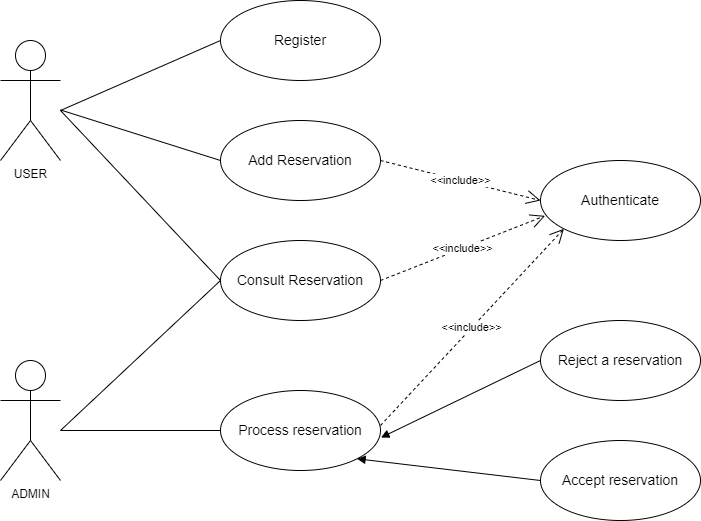
\includegraphics[width=6cm,height=6cm]{images/usecase.drawio.png}
    \caption{General use case diagram}
    \label{General use case diagram}
\end{figure}

In order to clarify the cases represented in the previous diagram, we create the following tables that contain a brief description of each use case. 
    
\textbf{• \textbf{Textual description for the use case "authenticate" }}

\begin{table}
    \centering
    \begin{tabular}{|c|l|} \hline 
         Title& Authenticate\\ \hline 
         Resume& Allow platform users to authenticate to access it.\\ \hline 
         Actors& User and Admin\\ \hline 
         Precondition&The user already has an account.\\\hline \hline 
         Nominal scenario& 1- The user enters their email address and password.\\ \hline 
 &2- The system checks the existence of the account in the DB by email.\\ \hline 
 &3- The system verifies the correspondence of the email with the pwd.\\ \hline 
 &4- Upon success, the user is authenticated.\\\hline \hline 
         Alternate scenario& E1: Account not found\\ \hline 
 &1- The system displays an error message.\\
 &2- The scenario continues from 1-\\\hline \hline 
 &E2: Incorrect password\\ \hline 
 &1- The system displays an error message'incorrect pwd or email adr'.\\ \hline
    \end{tabular}
    \caption{Textual description for the use case "authenticate"}
    \label{Textual description for the use case "authenticate"}
\end{table}

\textbf{• \textbf{Textual description for the use case "Process reservation" }}

\begin{table}
    \centering
    \begin{tabular}{|c|l|} \hline 
         Title& Process reservation\\ \hline 
         Resume& Allow the application administrator to manage complaints.\\ \hline 
         Actors& Admin\\ \hline 
         Precondition&The user is authenticated as an administrator.\\\hline \hline 
         Nominal scenario& 1- Consult reservation list.\\ \hline 
 &2- Choose a reservation to edit.\\ \hline 
 &3- Change reservation status"In progress/closed/rejected".\\\hline
    \end{tabular}
    \caption{Textual description for the use case "Process reservation" }
    \label{Textual description for the use case "Process reservation" }
\end{table}

\textbf{• \textbf{Textual description for the use case "Add reservation" }}

\begin{table}
    \centering
    \begin{tabular}{|c|l|} \hline 
         Title& Add reservation\\ \hline 
         Resume& Allow platform users to add reservation.\\ \hline 
         Actors& User \\ \hline 
         Precondition&The user is authenticated as a client\\\hline \hline 
         Nominal scenario& 1- The user clicks on "add resrvation"\\ \hline 
 &2- The system displays the reservation form\\ \hline 
 &3- The user fills out the form\\ \hline 
 &4- The user clicks on submit\\ \hline 
 &5- If successful, the reservation is successfully added.\\\hline \hline 
         Alternate scenario& E1: A field in the form is missing\\ \hline 
 &1- The system displays an error message indicating the problem.\\ \hline 
 &2- The user rectifies the error, and the scenario continues from 3.\\ \hline
    \end{tabular}
    \caption{Textual description for the use case "Add reservation"}
    \label{Textual description for the use case "Add reservation"}
\end{table}

\textbf{• \textbf{Textual description for the use case "Register " }}

\begin{table}
    \centering
    \begin{tabular}{|c|l|} \hline 
         Title& Register\\ \hline 
         Resume& Allow platform users to create an account.\\ \hline 
         Actors& User \\ \hline 
         Precondition&User have no account\\\hline \hline 
         Nominal scenario& 1- The user clicks on "Create account"\\ \hline 
 &2- The system displays the account creation form\\ \hline 
 &3- The user fills out the form and clicks on submit\\ \hline 
 &4- The system validate informations and inputs \\ \hline 
 &5- If successful, the account is successfully created.\\\hline \hline 
         Alternate scenario& E1: A field in the form is missing\\ \hline 
 &1- The system displays an error message indicating the problem.\\ \hline 
 &2- The user rectifies the error, and the scenario continues from 3.\\ \hline
 &E2: The client cancels\\\hline
    \end{tabular}
    \caption{Textual description for the use case "Register "}
    \label{Textual description for the use case "Register"}
\end{table}

\textbf{• \textbf{Textual description for the use case "Consult reservation " }}

\begin{table}
    \centering
    \begin{tabular}{|c|l|} \hline 
         Title& Consult reservation\\ \hline 
         Resume& Allow application users to view reservations.\\ \hline 
         Actors& User and Admin\\ \hline 
         Precondition&The user is authenticated\\\hline \hline 
         Nominal scenario& 1- if User : consult his own reservations\\ \hline 
 &2- if Admin : consult all reservations\\\hline
    \end{tabular}
    \caption{Textual description for the use case "Consult reservation "}
    \label{Textual description for the use case "Consult reservation"}
\end{table}


\section{Conclusion}
This chapter allowed us to cover the various functional and non-functional requirements that our solution must meet. We have also detailed these requirements through the use case diagram, in order to proceed to the design of our application, which will be presented in the next chapter. 
\chapter{Architecture and Design }

\section{Introduction }
In this chapter, we will embark on a crucial part of software development that bridges the gap between specification and implementation. This entails the design of the application. We will first present the general design of our application, followed by the detailed design including static views through class diagrams and dynamic views through sequence diagrams. 

\section{Architecture  }

• \textbf{MVC Architecture} 

The Model-View-Controller or MVC is a software architectural pattern intended for graphical interfaces, launched in 1978 and widely popular for web applications. The pattern consists of three types of modules with three different responsibilities: models, views, and controllers.

\begin{itemize}
    \item A model (Model) contains the data to display.
    \item A view (View) contains the presentation of the graphical interface.
    \item A controller (Controller) contains the logic concerning the actions performed by the user.
\end{itemize}
 
\begin{figure}[H]
   \centering
    %\includegraphics[scale=0.5]{images/trasfvs.jpg}
    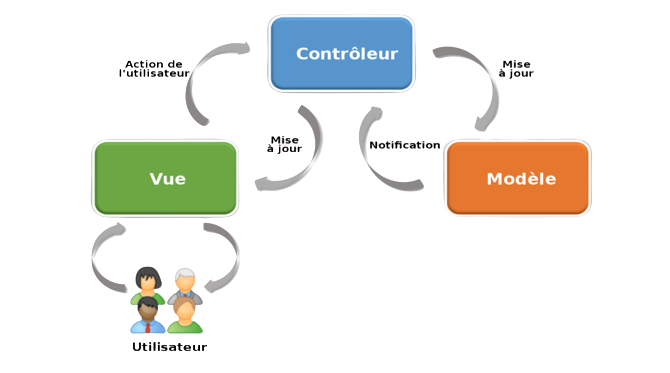
\includegraphics[width=15cm,height=8cm]{images/MVC.png}
    \caption{MVC Architecture} 
    \label{MVC Architecture}
\end{figure}

\section{Application mockups   }

"Authentication Mockup" To access the application, the user must either authenticate or sign up. 

\begin{figure}[H]
   \centering
    %\includegraphics[scale=0.5]{images/trasfvs.jpg}
    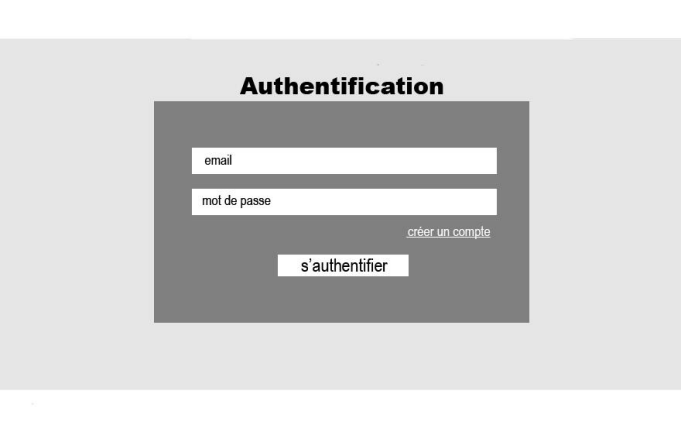
\includegraphics[width=15cm,height=8cm]{images/maqauth.png}
    \caption{Authentication Mockup} 
    \label{Authentication Mockup}
\end{figure}

"Sign Up Mockup" To access the application, the user must create an account. 

\begin{figure}[H]
   \centering
    %\includegraphics[scale=0.5]{images/trasfvs.jpg}
    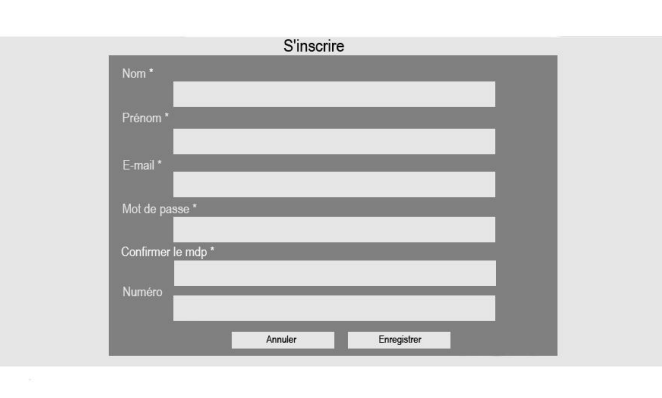
\includegraphics[width=15cm,height=8cm]{images/maqinsc.png}
    \caption{Sign Up Mockup} 
    \label{Sign Up Mockup}
\end{figure}




\section{Detailed design   }
\subsection{Class diagram  }

The class diagram is a static representation of the elements that make up a system and their relationships. The figure includes the main classes of our application and their associations. 

\begin{figure}[H]
   \centering
    %\includegraphics[scale=0.5]{images/trasfvs.jpg}
    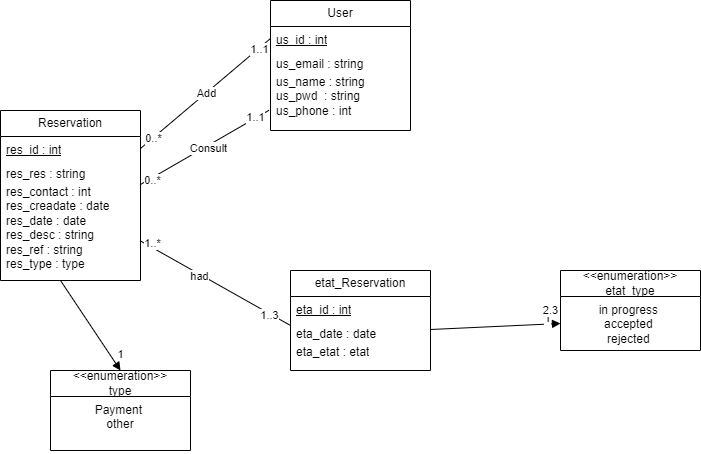
\includegraphics[width=15cm,height=8cm]{images/class.drawio.png}
    \caption{Class diagram} 
    \label{class diagram}
\end{figure}

\subsection{Sequence diagrams   }
The sequence diagrams provide a dynamic view of the interaction between the actor and the system. In this section, we represent the sequence diagrams related to some usage scenarios of our system .
    \item \textbf{Sequence diagram: Authentication }
\begin{figure}[H]
   \centering
    %\includegraphics[scale=0.5]{images/trasfvs.jpg}
    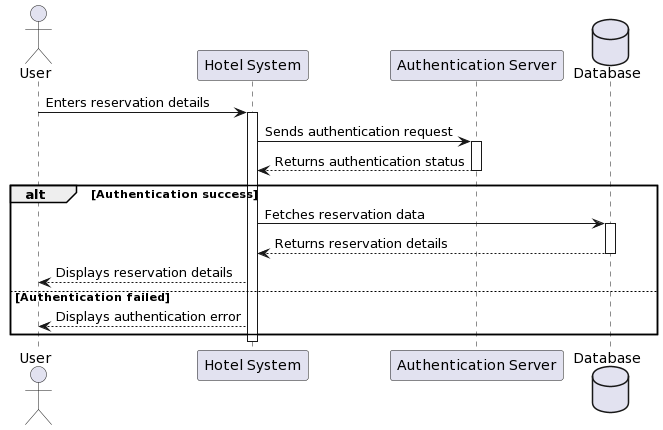
\includegraphics[width=15cm,height=8cm]{images/seq.png}
    \caption{Sequence diagram: Authentication } 
    \label{Sequence diagram: Authentication }
\end{figure}
\item \textbf{Sequence diagram: Manage reservation}

\begin{figure}[H]
   \centering
    %\includegraphics[scale=0.5]{images/trasfvs.jpg}
    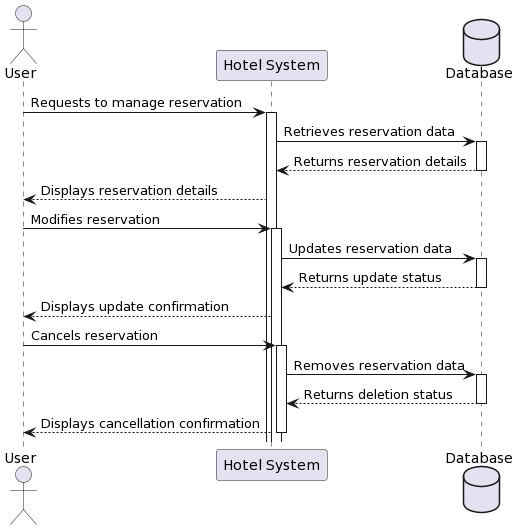
\includegraphics[width=15cm,height=8cm]{images/seq2.png}
    \caption{Sequence diagram: Manage reservation } 
    \label{Sequence diagram: Manage reservation  }
\end{figure}

\subsection{Activity diagram    }

This activity diagram provides a view of the behavior of a system by describing the sequence of actions in a process. 
\begin{figure}[H]
   \centering
    %\includegraphics[scale=0.5]{images/trasfvs.jpg}
    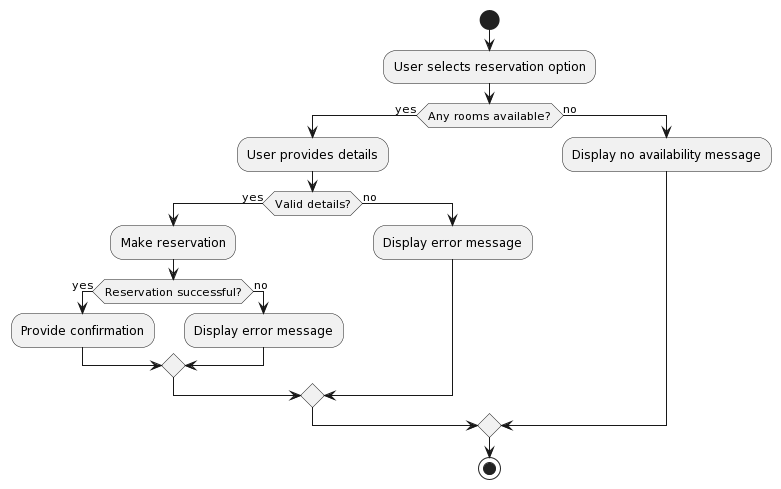
\includegraphics[width=15cm,height=8cm]{images/act.png}
    \caption{Activity diagram : manage reservation } 
    \label{activity diagram : manage reservation }
\end{figure}

\section{Conclusion }
Through this chapter, we have established the design of our application. Firstly, we began by outlining the architecture of our work, then we presented the class diagram that we deemed necessary to understand the functioning of our application. With the design of our module established, we now move on to the implementation phase. 
\chapter{Realization }

\section{Introduction}

After completing the design phase, we embark on the implementation phase in this chapter. We will begin by presenting the working environment used for development. Then, we will provide an overview of the work accomplished on the developed application. 

\section{Working environment }

\subsection{Hardware environment }

In order to develop our module under the most favorable conditions, we have made available a computer with the following configuration: 
• PC GIGABYTE G5 GE : Intel Core i5-12500H (Up to 4,50 GHz Turbo max, 18 Mo of memory cache, 12-Cores)  with 16GB of RAM
• Operating System: Windows 11 pro 
• Hard disk space: 512 GB SSD

\subsection{Software environment }

In order to develop our application, we have chosen to use the following software environment:

• \textbf{Visual Studio Code:} Visual Studio Code is an extensible code editor developed by Microsoft for Windows, Linux, and macOS. Features include debugging support, syntax highlighting, intelligent code completion, snippets, code refactoring, and integrated Git. 

\subsection{Framework }

        \item \textbf{Angular 14.7.0:} Angular is an open-source client-side framework based on TypeScript, co-led by the Angular team at Google and a community of individuals and corporations. Angular is a complete rewrite of AngularJS, a framework built by the same team. 
        \item \textbf{Spring  Boot 2.7.3:}Spring Boot is a new framework created by the team at Pivotal, designed to simplify the startup and development of new Spring applications. 
\item \textbf{Bootstrap 5.0:} Bootstrap is a collection of tools useful for creating the design (graphics, animations, and page interactions in the browser, etc.) of websites and web applications. It is a set that contains HTML and CSS code, forms, buttons, navigation tools, and other interactive elements, as well as optional JavaScript extensions. 

\subsection{Data Base : MySql  }

\textbf{MySQL} is a relational database management system (RDBMS). It is distributed under a dual GPL and proprietary license. It is one of the most widely used database management software in the world, both by the general public (mainly web applications) and professionals, competing with Oracle, PostgreSQL, and Microsoft SQL Server. 

\section{Work accomplished  }

This section is dedicated to presenting the interfaces of the application developed during this project. 

\subsection{The interfaces of the application  }

•\textbf{ Authentication interface  :}
To log in, the client must enter their email address and password. In the case where the client is not registered, they must create an account. To add a reservation, the user presses the 'add a new reservation button, where they will be redirected to the reservation submission interface. 
 \begin{figure}[H]
   \centering
    %\includegraphics[scale=0.5]{images/trasfvs.jpg}
    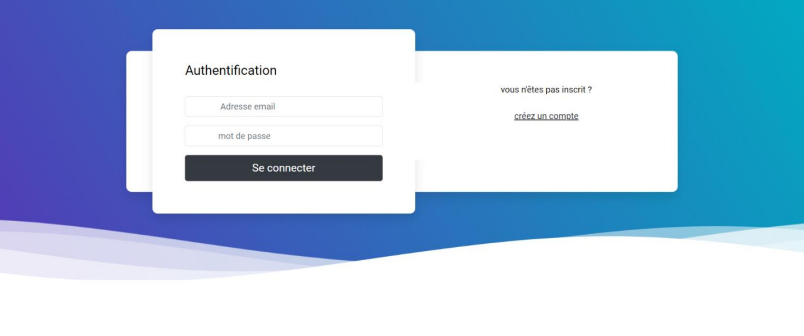
\includegraphics[width=15cm,height=8cm]{images/autint.png}
    \caption{Authentication interface } 
    \label{Authentication interface }
\end{figure}

•\textbf{ Account Creation Interface   :}

Once the client clicks on the 'create an account' link, a form will be displayed for them to create their account by filling out the form with their personal information. 
 \begin{figure}[H]
   \centering
    %\includegraphics[scale=0.5]{images/trasfvs.jpg}
    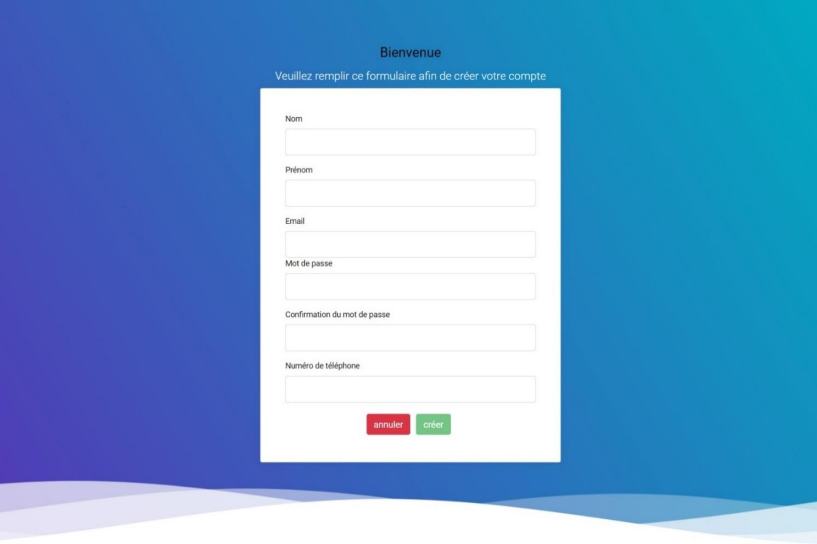
\includegraphics[width=15cm,height=8cm]{images/inscit.png}
    \caption{Account Creation Interface } 
    \label{Account Creation Interface }
\end{figure}


•\textbf{ Admin Interface   :}

\begin{figure}[H]
   \centering
    %\includegraphics[scale=0.5]{images/trasfvs.jpg}
    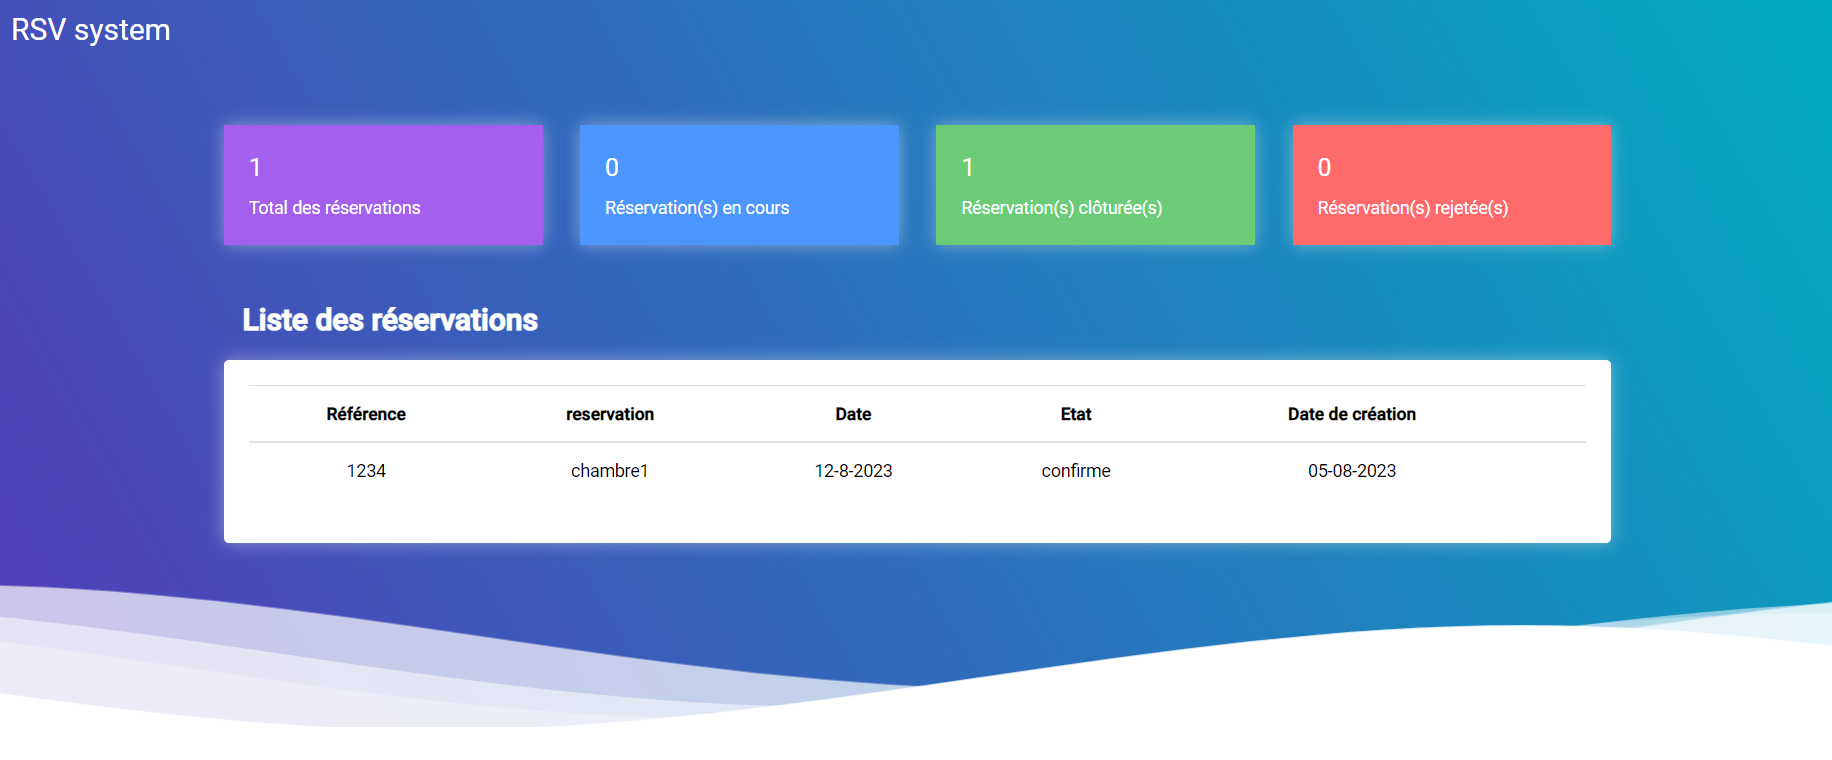
\includegraphics[width=15cm,height=8cm]{images/consint.png}
    \caption{Admin Interface } 
    \label{Admin Interface }
\end{figure}







\section{Conclusion}
This chapter presents the final phase of the project development, which is the implementation phase. Firstly, we defined the working environment and the technologies used, then we presented some screenshots. Finally, we will conclude our report with the consolidated achievements and a general conclusion. 
\chapter*{General Conclusion}
\addcontentsline{toc}{chapter}{General Conclusion}
This internship has been very enriching for me as it allowed me to consolidate my design skills, enrich my knowledge in JAVA, and learn Angular, which is a very comprehensive and powerful framework. This internship also offered me the opportunity to discover and work with the MySQL relational database management system.

With this experience and in response to its challenges, I would like to try adding a module where the administrator can manage complaints. In this stage, we have completed our project, but this does not imply that the work done is perfect or unchangeable. On the contrary, it will remain open to any proposals for improvement.

 

 




%récupérer les citation avec "/footnotemark"
\nocite{*}

%choix du style de la biblio
\bibliographystyle{acm}
%inclusion de la biblio
\bibliography{references.bib}

\end{document}
